\section{Proxy模块分析}

Proxy充当HSM命令派发与Copytool管理的功能,其主要架构如下:

\begin{figure}[!htb]
    \centering
    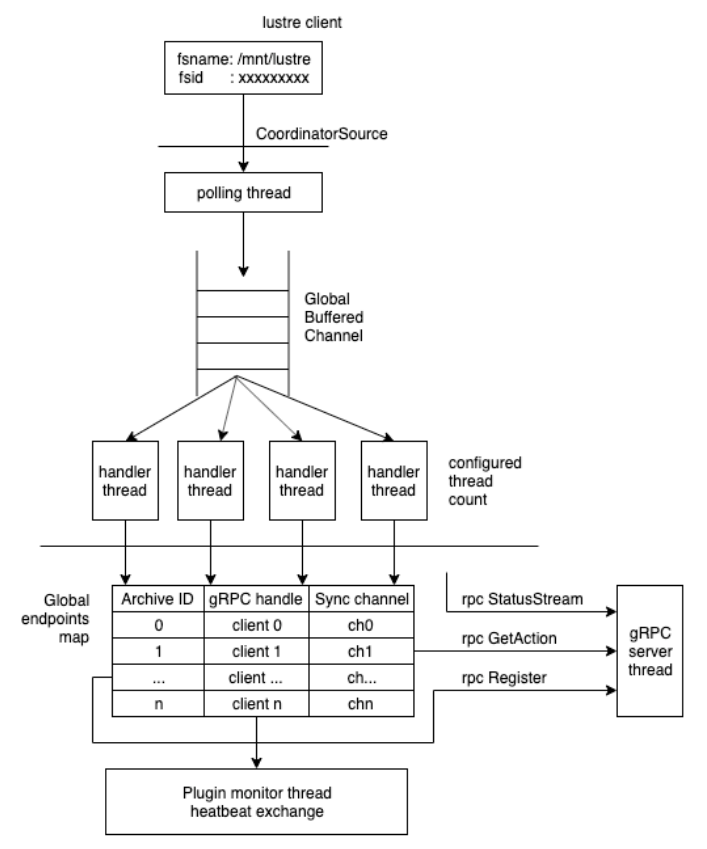
\includegraphics[width=0.9\linewidth]{proxy.png}
    \caption{Proxy模块}\label{fig:region-image}
\end{figure}

Proxy启动时首先加载配置文件,之后根据配置文件挂载lustre客户端,并创建以及注册lustre HSM的客户端。该客户端同时 又作为gRPC的服务端,管理DataMover客户端以及HSM命令的派发。创建HSM客户端之后,proxy会启动HSM poll线程以同步的方式接收来自lustre的HSM命令,并将这些命令放入一个全局队列中。之后启动一个或多个handler线程用于从全部队列中取出HSM命令,并放入对应的客户端的sync channel中。HSM同时会启动一个Plugin监控线程以及一个gRPC服务线程。Plugin监控线程用于周期性的确认每个DataMover实例是否工作正常,以及服务不可用时的处理办法。gRPC服务线程用于为gRPC客户端提供服务。gRPC服务启动时,会向外部导出三个服务接口: 

\subsection{rpc Register}
该rpc接口由DataMover调用,用于向Proxy注册一个DataMover实例。每个注册的DataMover实例都会按照Archive ID为索引的全部map中。每个DataMover实例在一个Proxy中必须唯一。通过Archive ID可以索引到对应的gRPC客户端handle,服务端可以通过该handle与gRPC客户端进行通信。另外,通过Archive ID也可以获取对应到该客户端的sync channel,每个派发到该客户端的HSM命令都会放到该channel中。channel中的HSM命令并不会由Proxy主动推送到客户端中,必须由客户端主动调用rpc GetAction获取对应的HSM命令。 

\subsection{rpc GetAction}

客户端主动调用该rpc,用户同步的获取属于该客户端的HSM命令。如果不存在发往该客户端的命令,则该客户端会被阻塞。如果Proxy端存在发往该客户端的HSM命令,则Proxy会调用rpc Send将sync channel的HSM命令取出并发往对应的客户端。 

\subsection{rpc StatusStream}

该rpc调用用于DataMover实例向Proxy汇报数据搬运的进度,Proxy接收 到进度信息时会进度进一步封装并发回到CDT服务中,CDT服务根据进度信息可以间接确认Proxy的活动状态。 

Global endpoints map是Proxy中重要的数据结构。客户端主动调用Register时Proxy会在该map中登记客户端对应的信息。Plugin monitor监测到客户端DataMover出现不可恢复异常时,会将对应的客户端项从该表中删除。 

